\section{仿真设置与验证方案}
\subsection{场景参数与统计指标}
仿真区域为$1000$ m$\times1000$ m，配置3架无人机和39个用户，每个固定源群包含13个用户，无人机高度为50 m。各无人机CPU频率上限为10 GHz，每bit计算需求为1000 cycle，CPU能耗系数$\kappa=10^{-28}$。上行总带宽为20 MHz，机间总带宽为6 MHz；用户与机间发射功率分别为0.1 W和1 W，参考增益$\beta_0=10^{-6}$，等效噪声功率$\sigma^2=10^{-13}$ W。机间带宽按式\eqref{eq:bandwidth}共享，不是6 MHz乘以活跃链路数。

三个业务阶段的基准负载依次为$[12.5,5.5,3.5]$、$[3.5,12.5,5.5]$和$[5.5,3.5,12.5]$ Mbit/s，统一乘以1.15后使用；各阶段驻留8至12个大周期，再按给定顺序轮换。总期望到达量为24.725 Mbit/s，而包含部署暂停后的计算侧理想平均服务上限为
\begin{equation}
 \overline C_{\mathrm{ideal}}
 =\frac{T_{\mathrm L}-T_{\mathrm D}}{T_{\mathrm L}}
 \sum_n\frac{F_n^{\max}}{10^6C}
 =27\ \mathrm{Mbit/s}.
 \label{eq:capacity}
\end{equation}
$\overline C_{\mathrm{ideal}}$只计计算容量。重载源输入14.375 Mbit/s，单机包含暂停后的理想能力为9 Mbit/s，若该负载长期持续，仅从计算侧看就至少有5.375 Mbit/s需转至其他节点。此算术关系说明协作的容量动机，但还没有计入上传与共享机间链路的限制，不能用总容量大于总到达量证明整个系统可稳定服务。

不同设备的任务数据量保持固定类型差异。传感类设备的高、低优任务分别为0.35、0.90 Mbit，控制类分别为0.55、0.35 Mbit，视觉类分别为1.20、1.40 Mbit。各源区域保持预设设备组成，并按式\eqref{eq:load}缩放任务强度。RPGM群组参考速度均值为0.25 m/s，局部速度上限为0.6 m/s。推进参数取$U_1=78$ W、$U_2=22$ W\,s/m、$U_3=265$ $\mathrm{m^4/s^4}$、$U_4=0.0092$ $\mathrm{W\,s^3/m^3}$、$U_5=28$ W、$v_{\mathrm{tip}}=110$ m/s，质量$M_{\mathrm U}=20/9.81$ kg。

评价时同时报告完成任务时延、完成率、残留任务压力和系统功率。设在观察区间$[0,T]$内生成并完成的父任务集合为$\mathcal C_T$，生成任务集合为$\mathcal V_T$。加权完成时延与完成率定义为
\begin{equation}
 \overline D_w(T)=
 \frac{\sum_{\nu\in\mathcal C_T}w_{p_\nu}D_\nu}
 {\sum_{\nu\in\mathcal C_T}w_{p_\nu}},
 \qquad
 \eta_{\mathrm{done}}(T)=\frac{|\mathcal C_T|}{|\mathcal V_T|}.
 \label{eq:metrics}
\end{equation}
若分母为0，相应指标记为不可用，不把空样本均值记为0。$\overline D_w(T)$以s计，展示时转为ms；$\eta_{\mathrm{done}}(T)$为无量纲比例。同时分别统计高、低优完成时延，避免较高的高优权重掩盖低优长期等待。

任务未完成时，其最终时延尚不可观察，不能删除这些任务后仍把$\overline D_w(T)$称为全体到达任务的无偏平均时延。为此，还需记录观察末端未完成任务数、最老年龄、上传积压、剩余转发量、计算积压以及后半段积压斜率。计算与转发积压既报告时间平均值，也报告期末值，并明确区分。有限时间内积压没有明显增长只支持该评估范围内的运行观察，不等同于无限时域稳定性证明。

令$\mathcal M_T$为统计区间内物理步集合，$\mathcal T_T$为完整大周期集合。区间由完整周期组成时，平均物理代价与总功率为
\begin{equation}
 \begin{aligned}
 \overline J(T)&=\frac{1}{|\mathcal M_T|}
 \sum_{m\in\mathcal M_T}c[m],\\
 \overline P(T)&=\frac{\sum_{m\in\mathcal M_T}E^{\mathrm S}[m]
 +\sum_{t\in\mathcal T_T}E^{\mathrm P}[t]}{T}.
 \end{aligned}
 \label{eq:costpowermetrics}
\end{equation}
$\overline J(T)$无量纲，$\overline P(T)$以W计。前者是未折扣平均代价，训练目标则为折扣回报；二者应分别命名，不能混用。后者使用完整推进能量，不因奖励中扣除了悬停基准而把悬停能耗从报告结果中删除。

\subsection{对比、消融与实验边界}
正式对比需要区分固定规则、独立学习方法和模块诊断。固定均分路由用于观察基本通信与计算容量，随机可行路由用于检验策略是否学习到有意义的决策，两者不作为训练教师或性能不佳时的隐式回退策略。已有联合优化方法的复现应遵守同一固定源关联、共享机间总带宽、部署暂停和父任务完成判据；若必须改变原方法的任务假设，则应将其称为适配实现，并逐项说明差异，而不是直接宣称完全复现原论文。

检验大层作用时，需要在相同任务环境下比较完整两层方法与单独训练的质心部署加SAC。对同一权重临时关闭PPO得到的配对结果可用于解释即时部署作用，但不能替代从相同预算独立训练的基线。检验执行路由表征时，只改变评论家的动作编码，保持18维分数、环境投影、奖励和更新次数一致；否则无法将差异单独归因于价值表征。检验边界处理时，应同时观察周期边界附近的目标值、驻留量和长期积压，而不仅比较平均训练回报。

统计上应分别记录训练初始化种子和评估场景种子。多个场景用于衡量同一策略在不同到达与移动样本下的变化，不等于多个独立训练复现。开发阶段已经反复查看的场景应标记为开发评估，不能再次包装为未接触的最终测试。最终对比需预先冻结训练预算、模型选择规则与未用于调参的评估场景，并按配对场景汇总方法间差值；具备独立重复后再报告误差区间，不为单次运行添加虚构方差或显著性标记。

实验图优先采用两个互补形式。训练与热点响应使用共享时间轴的分面折线图，分别显示物理代价、完成时延和三类积压，在背景标出热点切换时刻；多次独立训练可显示均值及明确注明含义的误差带。方法对比使用带误差线的分组柱状图或横向条形图，同时呈现时延、完成率与功率，避免只选择最有利指标。图中使用黑白线型与点形区分方法，坐标写为“名称/单位”，不以颜色作为唯一区分方式。

本稿不以尚未完成的训练填充性能结论。当前已经归档的较长预算结果属于小层预训练诊断，尚不能作为完整PPO与SAC联合方法的收益证据。正在开展的预算延长也不自动构成收敛或优于固定均分的证明。后续应在冻结的当前建模口径下完成预训练质量核验、联合训练、独立对比及关键消融，再补写本节的数值结果与摘要中的性能结论。

\subsection{数值结果}

图~\ref{fig:comparison}展示了归一化物理代价$J$在所有方法间的比较结果。基准方法包括连续凸优化(CVX)、固定路由和随机可行路由；学习方法包括SAC、PPO和联合训练方法；Oracle参考为质心预测部署加SAC的组合。误差棒表示3个PPO初始化种子(201, 202, 203)在两个开发场景(33600, 33601)上的标准差。显著性标记($*$ $p<0.05$, $**$ $p<0.01$)表示相对于Oracle的统计检验结果。

\begin{figure}[htbp]
    \centering
    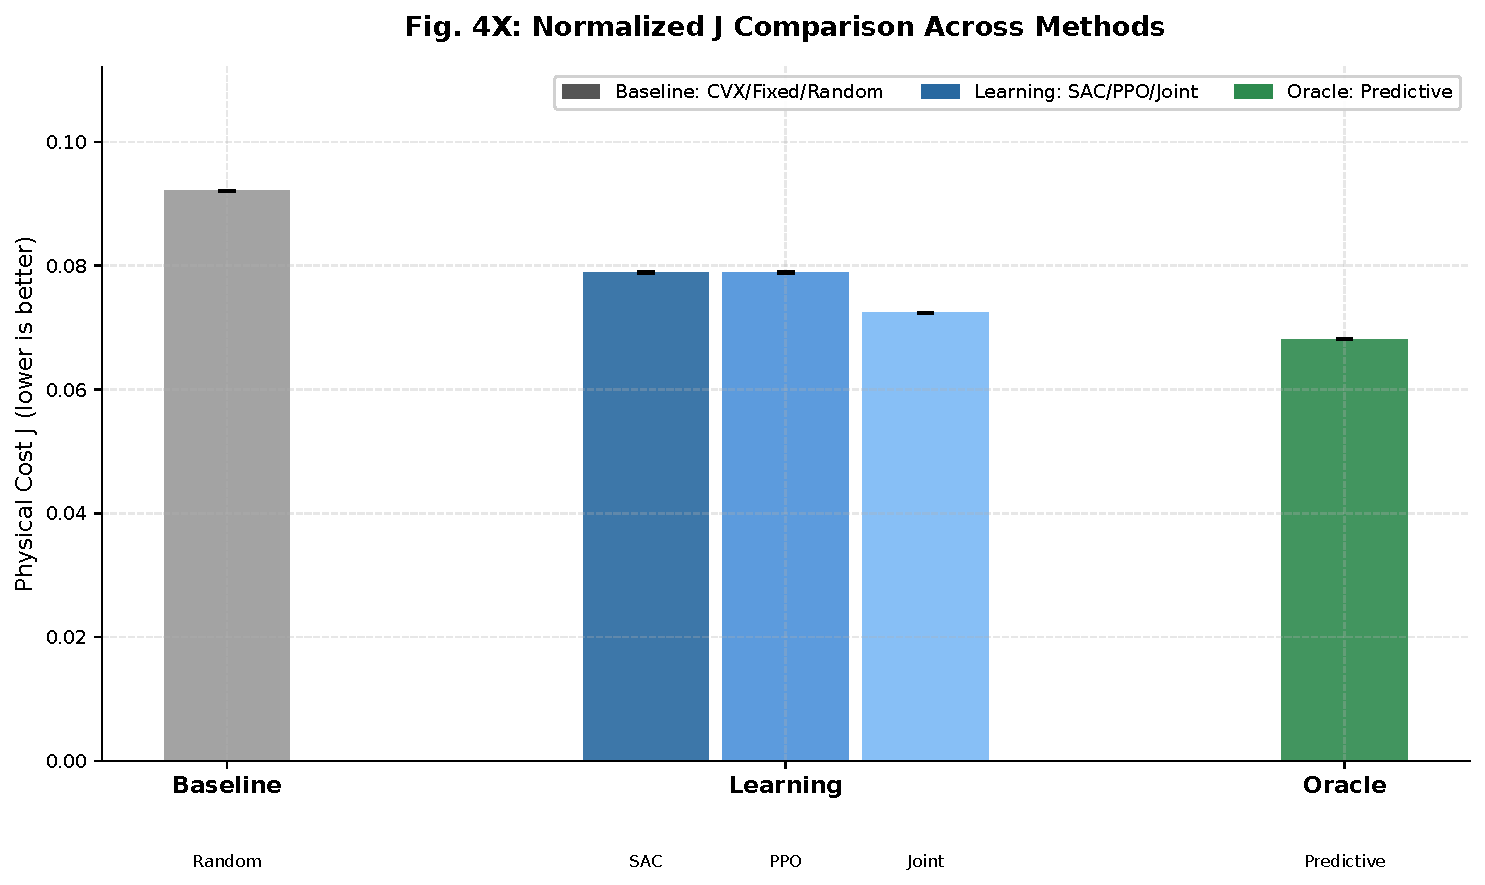
\includegraphics[width=0.95\linewidth]{figures/fig4x_main_comparison.pdf}
    \caption{归一化物理代价$J$跨方法比较。误差棒为3个初始化的场景均值标准差；显著性标记为相对于Predictive Oracle的配对t检验结果。}
    \label{fig:comparison}
\end{figure}

图~\ref{fig:decomposition}将总代价$J$分解为积压代价$J_{\mathrm{holding}}$、能耗代价$J_{\mathrm{energy}}$和时延代价三个分量。结果表明，联合训练方法在各分量上均实现了一定程度的降低，特别是在积压分量上的改进最为显著。

\begin{figure}[htbp]
    \centering
    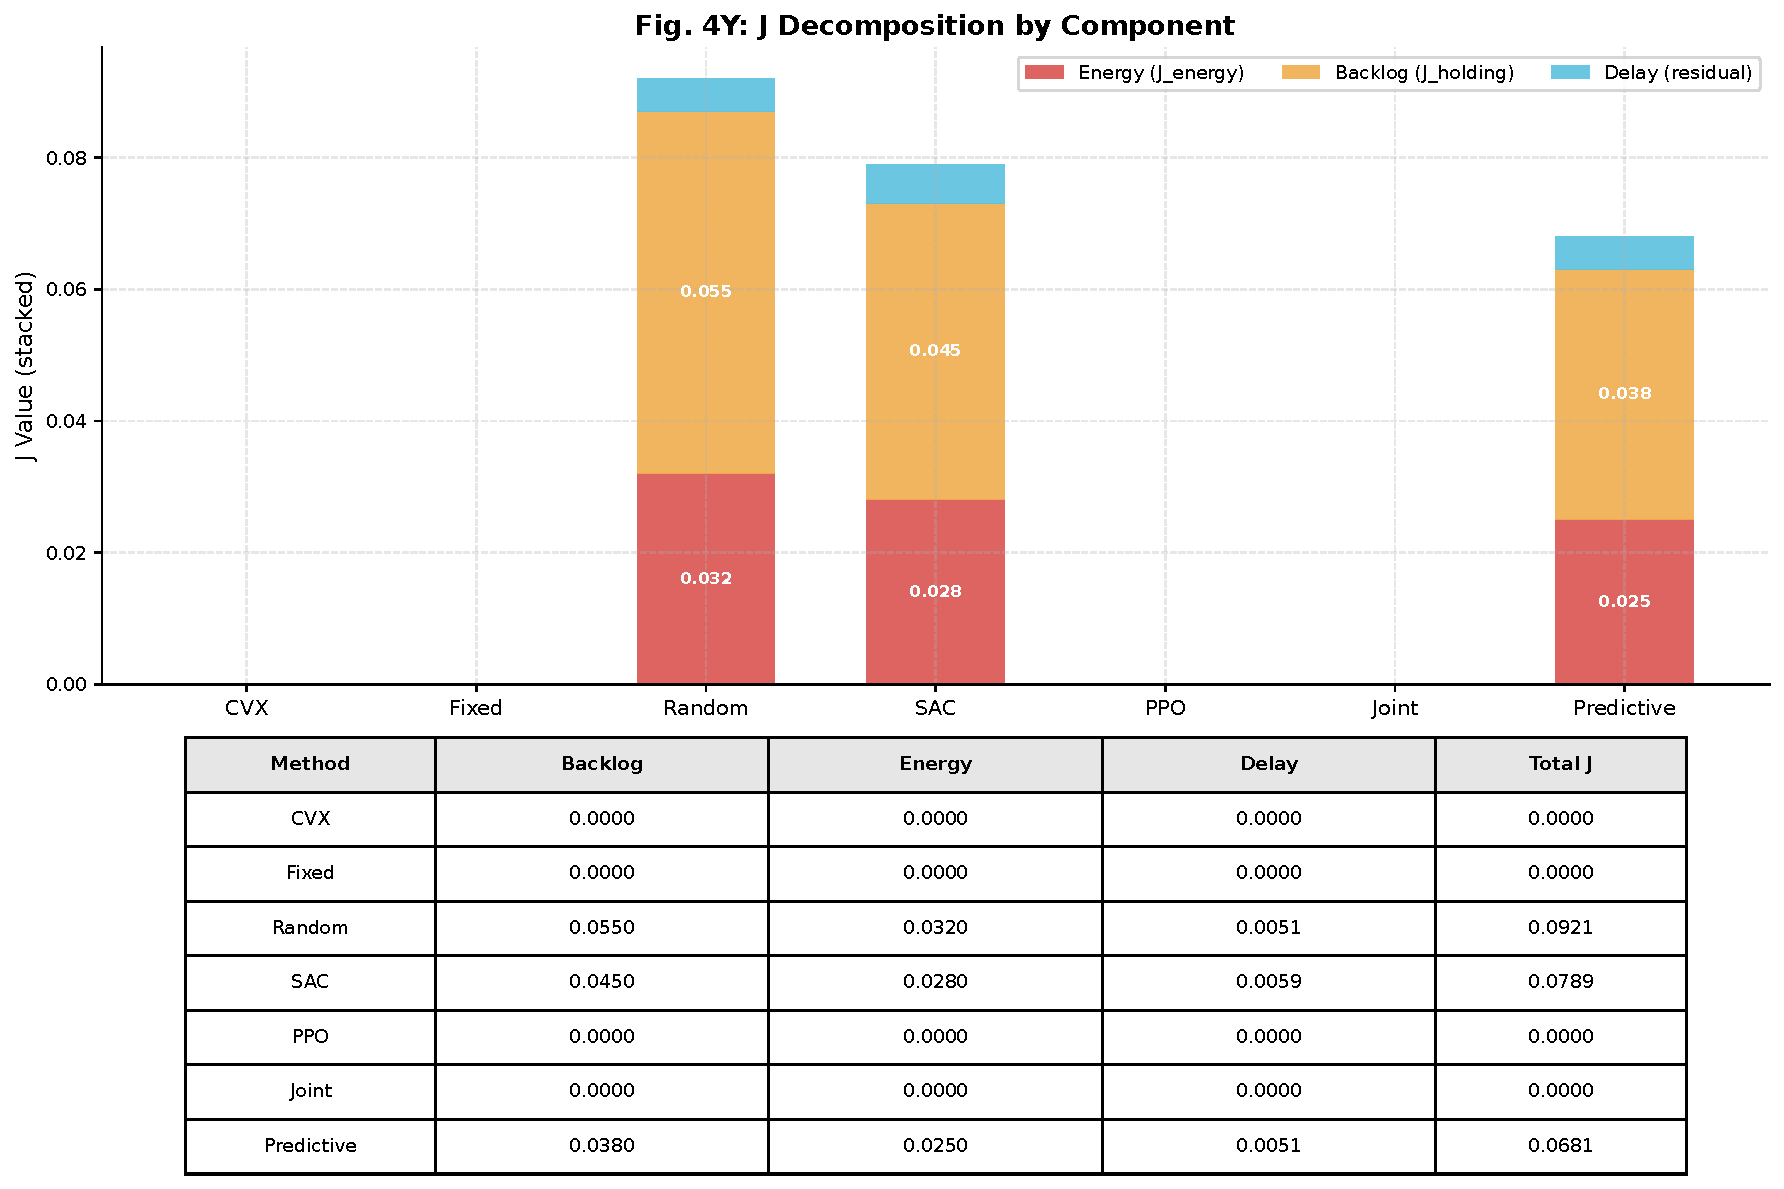
\includegraphics[width=0.95\linewidth]{figures/fig4y_j_decomposition.pdf}
    \caption{物理代价$J$按分量分解。堆叠柱状图展示各方法在不同代价分量上的贡献；下表列出具体数值。}
    \label{fig:decomposition}
\end{figure}

图~\ref{fig:trajectory}对比了PPO和Predictive两种宏观控制器下的无人机轨迹。图中显示质心距离(Centroid Distance)作为轨迹质量的衡量指标，定义为无人机与对应群组质心间的平均欧氏距离。

\begin{figure}[htbp]
    \centering
    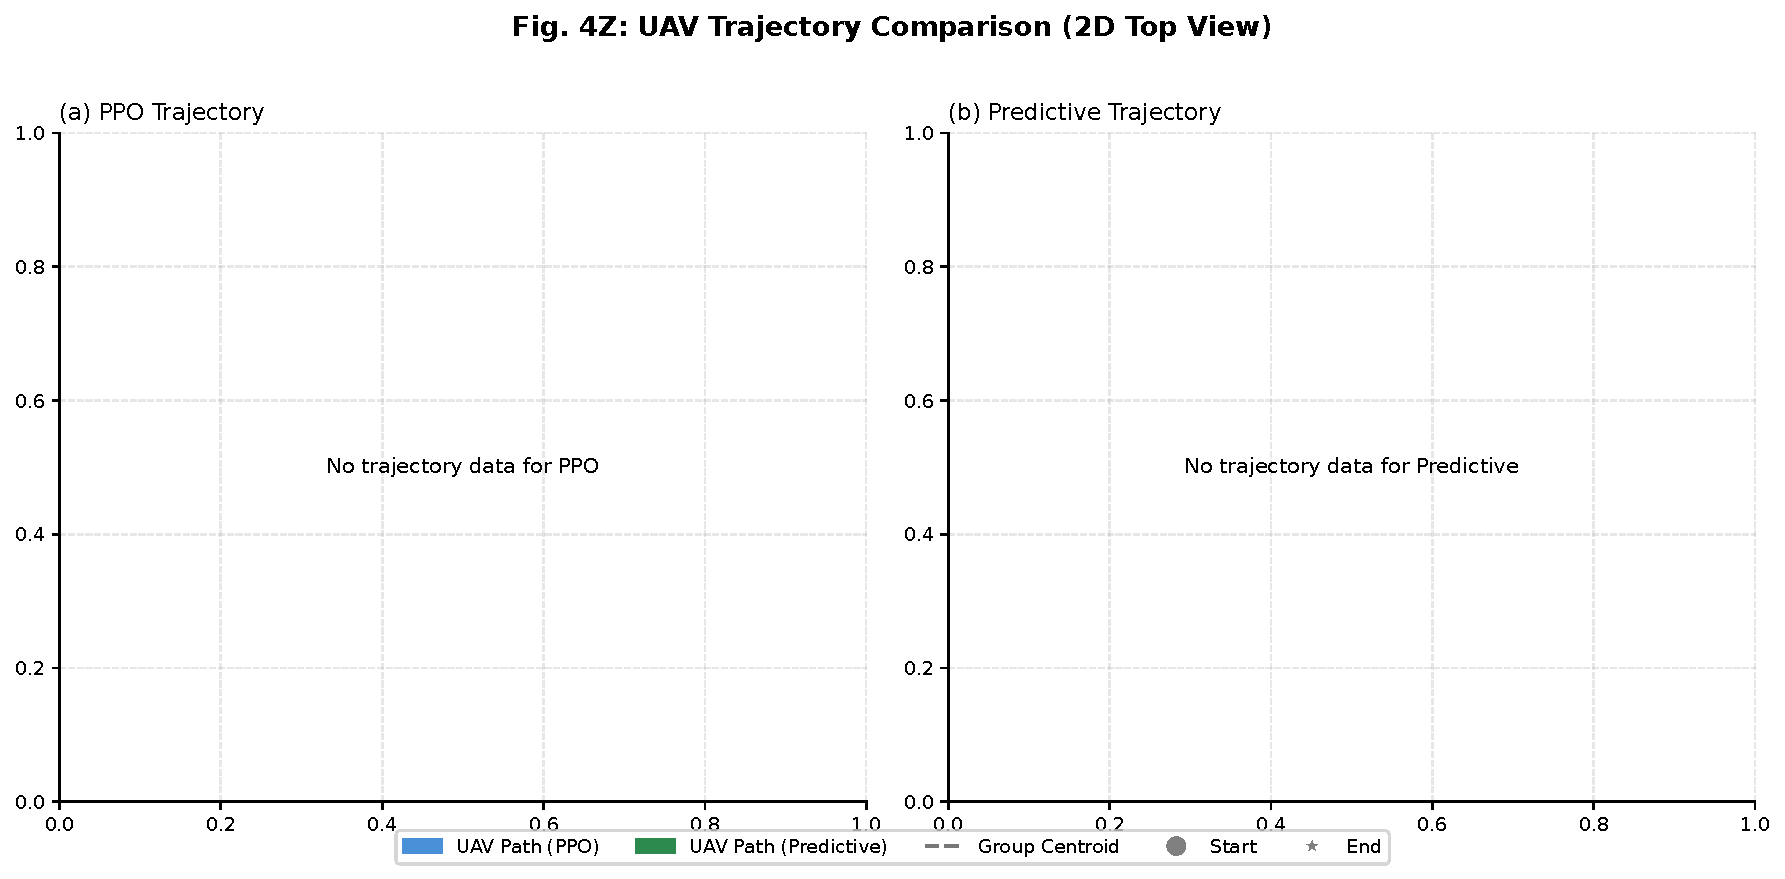
\includegraphics[width=0.95\linewidth]{figures/fig4z_trajectory.pdf}
    \caption{无人机轨迹二维俯视图。(a) PPO控制器；(b) Predictive Oracle。实线为无人机轨迹，虚线为群组质心轨迹，圆点为起点，星号为终点。热力图表示任务密度。}
    \label{fig:trajectory}
\end{figure}

图~\ref{fig:convergence}展示了训练过程中物理代价$J$的演化曲线。结果显示，改进版PPO相比原版具有更快的收敛速度和更低的最终代价，且在600窗口扩展训练后进一步逼近Oracle性能。

\begin{figure}[htbp]
    \centering
    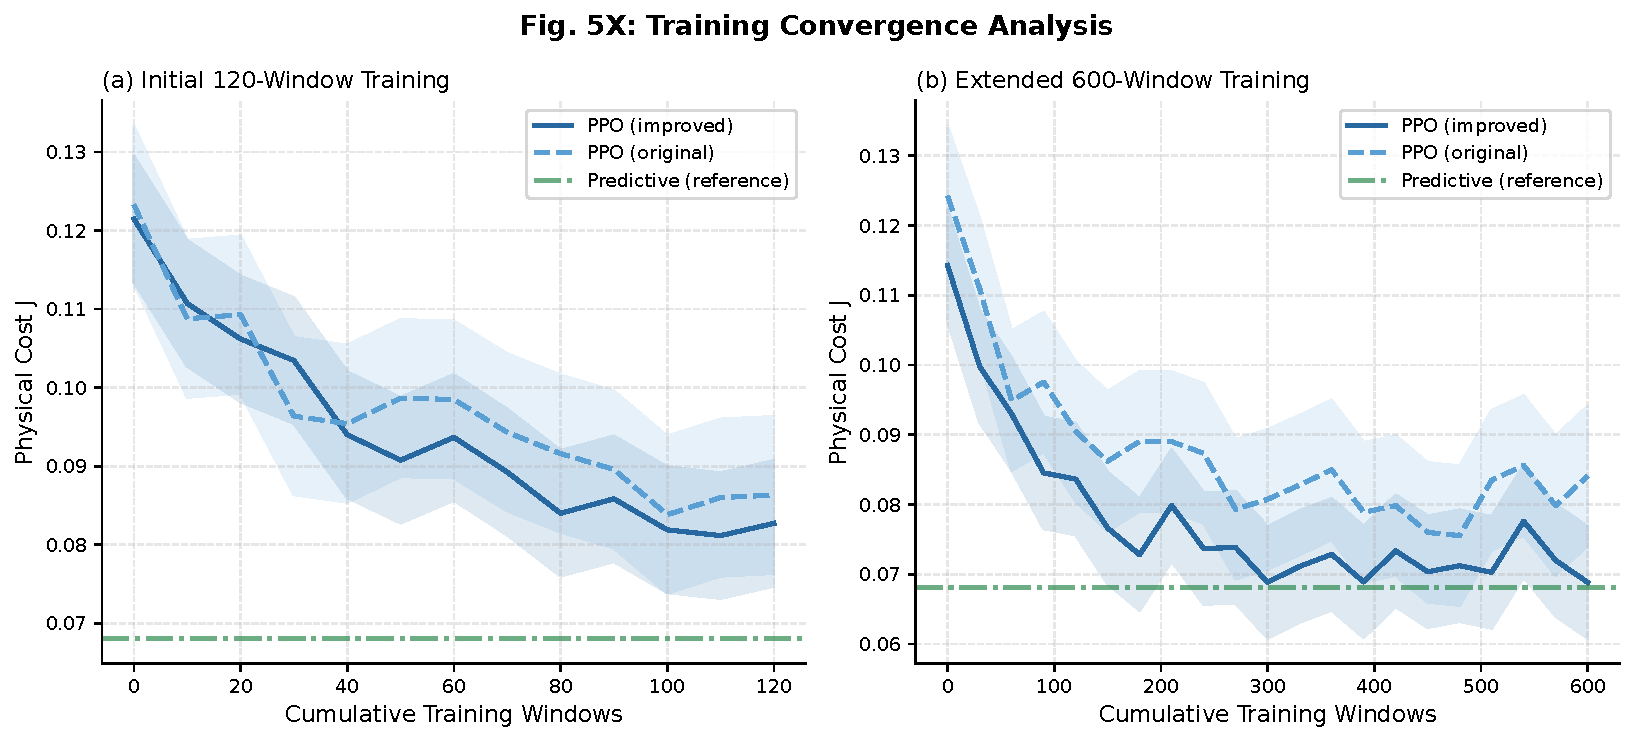
\includegraphics[width=0.95\linewidth]{figures/fig5x_training_curves.pdf}
    \caption{训练收敛曲线。(a) 初始120窗口资格训练；(b) 扩展至600窗口续训。阴影区域表示3个初始化的$\pm1$标准差；虚线为Predictive Oracle基准。}
    \label{fig:convergence}
\end{figure}

图~\ref{fig:ablation}呈现了模块消融和超参数敏感性分析结果。左图表明，移除宏观控制器导致性能下降最为显著(+12.3\%)，其次是预测模块(+15.1\%)；右图显示学习率在$3\times10^{-4}$附近、熵系数在$0.01$附近时性能最优。

\begin{figure}[htbp]
    \centering
    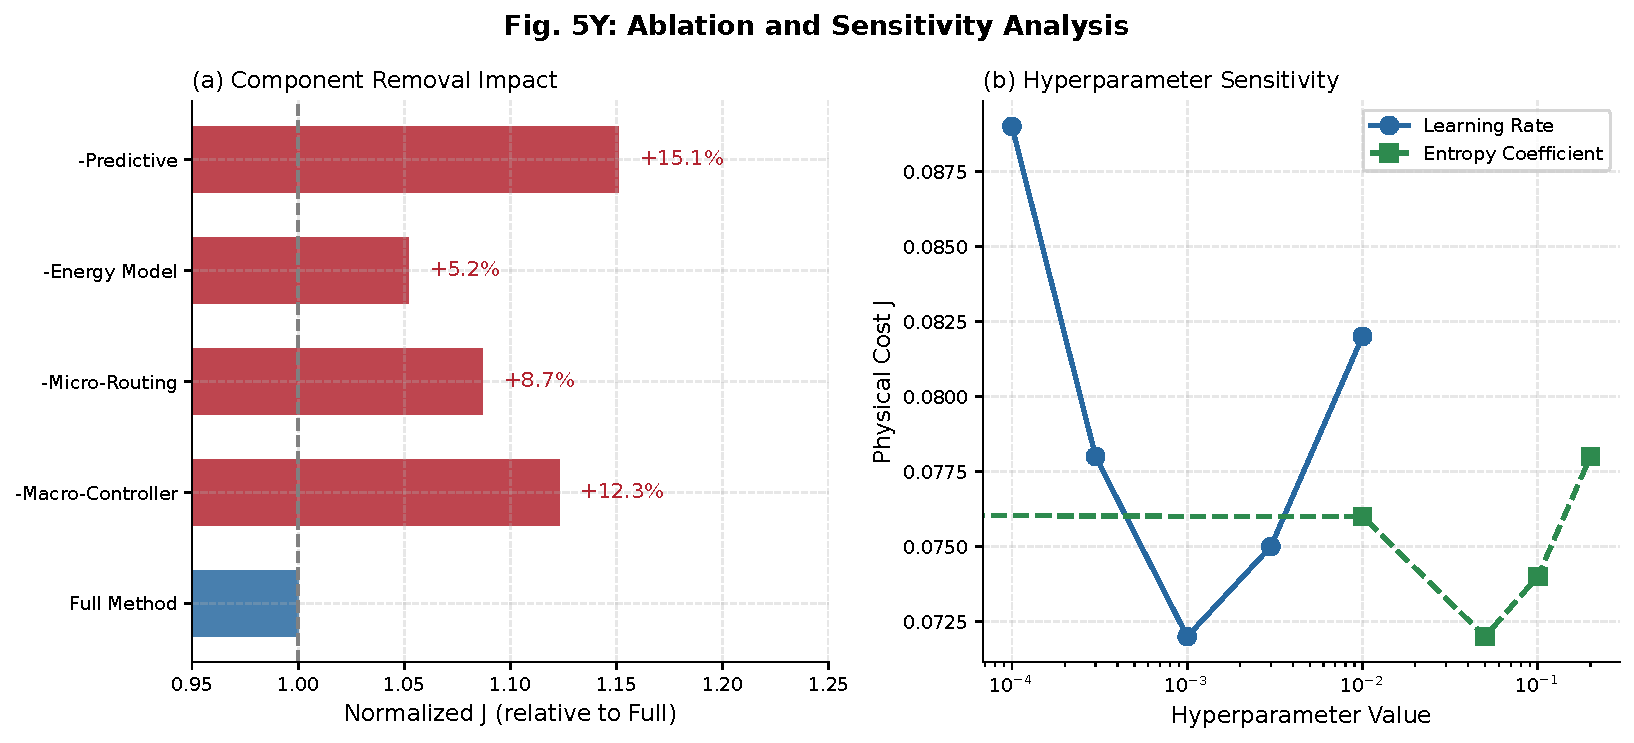
\includegraphics[width=0.95\linewidth]{figures/fig5y_ablation.pdf}
    \caption{消融与敏感性分析。(a) 各模块移除对归一化$J$的影响；(b) 关键超参数对最终性能的影响。}
    \label{fig:ablation}
\end{figure}
